\subsection{From a secant line to a tangent line}

For $f(x)=x^2$, the average rate of change between $x=1$ and $x=1+h$ is the slope of a secant line. As $h$ becomes smaller, the second point approaches the first and the secant approaches the tangent.

\begin{center}
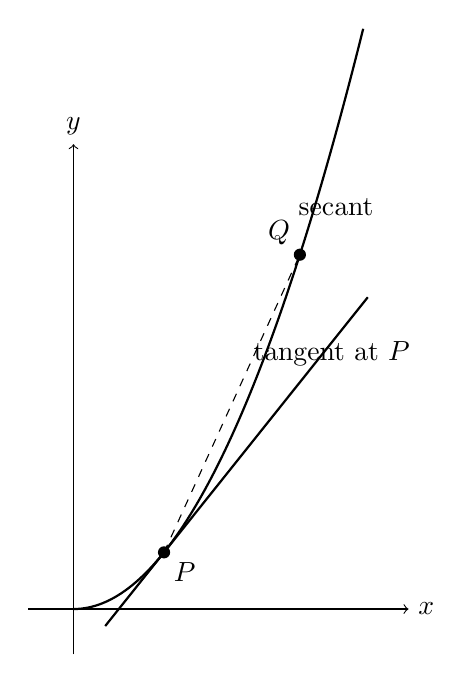
\begin{tikzpicture}[x=1.15cm,y=0.72cm]
  \draw[->] (-0.5,0) -- (3.7,0) node[right] {$x$};
  \draw[->] (0,-0.8) -- (0,8.2) node[above] {$y$};
  \draw[thick,domain=0:3.2,samples=80] plot (\x,{\x*\x});
  \fill (1,1) circle (2.2pt) node[below right] {$P$};
  \fill (2.5,6.25) circle (2.2pt) node[above left] {$Q$};
  \draw[dashed] (1,1) -- (2.5,6.25);
  \draw[thick] (0.35,-0.3) -- (3.25,5.5);
  \node at (2.9,7.1) {secant};
  \node at (2.85,4.5) {tangent at $P$};
\end{tikzpicture}
\end{center}

\begin{interpretationbox}[The derivative is a limiting slope]
The secant uses two points and gives an average rate of change. The tangent records the limiting position of those secants and gives the instantaneous rate of change at one point.
\end{interpretationbox}
